\begin{figure}[H]
  \begin{circuitikz}\draw
    (0,5) -- ++ (0.5,0)
    (0,5) to[short] (0,4.83)
    (0,4.5) circle ( 0.33 cm)
    (0,4.5) node {$e_1$}
    (0,4.16)  to[short] (0,4)
    (0,4) to[R,l=$r_\phi$] (0,3)
    (0,3) to[L,l=$L_\phi$] (0,2)
    (0,2)  to[Ty,l=$\!V_1$] (0,1)
    -- ++ (0,-1)
    -- ++ (0.5,0)
    %
    (1.2,5) to[short,-*] ++ (0.5,0)
    to[short,-*] ++ (1.4,0)
    (1.7,5) to[short] ++ (0,-0.17)
    (1.7,4.5) circle ( 0.33 cm)
    (1.7,4.5) node {$e_k$}
    (1.7,4.16)  to[short] ++ (0,-0.16)
    to[R,l=$r_\phi$] ++ (0,-1)
    to[L,l=$L_\phi$] ++ (0,-1)
    to[Ty,l=$\!V_k$] ++ (0,-1)
    to[short,-*] ++ (0,-1)
    -- ++ (0.8,0)
    (1.2,0) to[short] ++ (0.9,0)
    %
    (3.1,5) -- ++ (0.5,0)
    (3.1,5) to[short] ++ (0,-0.17)
    (3.1,4.5) circle ( 0.33 cm)
    (3.1,4.5) node {$e_{k\!+\!1}$}
    (3.1,4.16)  to[short] ++ (0,-0.16)
    to[R,l=$r_\phi$] ++ (0,-1)
    to[L,l=$L_\phi$] ++ (0,-1)
    to[Ty,l=$\!V_{k\,+\,1}$] ++ (0,-1)
    to[short,-*] ++ (0,-1)
    -- ++ (0.5,0)
    (2.5,0) to[short] ++ (0.5,0)
    %
    (5,5) to[short] ++ (0,-0.17)
    (5,4.5) circle ( 0.33 cm)
    (5,4.5) node {$e_{m}$}
    (5,4.16)  to[short] ++ (0,-0.16)
    to[R,l=$r_\phi$] ++ (0,-1)
    to[L,l=$L_\phi$] ++ (0,-1)
    to[Ty,l=$\!V_{m}$] ++ (0,-1)
    -- ++ (0,-1)
    %    -- ++ (0.5,0)
    (4.5,0) to[short,-*] ++ (0.5,0)
    %
    -- ++ (0.5,0)
%   
    (5.5,5) to[short,-*] ++ (-0.5,0)
    -- ++ (-0.5,0)
    ;\end{circuitikz}
\end{figure}

по госту обозначение диода
\begin{circuitikz}\draw
(0,0) to[Do] (1,0)--(0,0)
  ;\end{circuitikz}.

\begin{circuitikz}
  \draw[thin,->](0,0)--(2,0) node[right] {$\omega t$}
  ;\end{circuitikz}

Значения по оси времени откладываются в угловых единицах $\omega t$.
$\displaystyle{\frac{1}{50}\textcyrillic{сек}} $ -- период. $1msec= 18^\circ$

\begin{circuitikz}\begin{scope}[xscale=2,yscale=3]
    \draw[thin,->] (-pi/2,0) -- (pi+pi/2+pi/12,0) node[right] {$\omega t$};
    \draw[thin,->] (0,-1.1) -- (0,1.2) node[left] {U};

    \draw[thin,dotted,help lines,smooth] (-pi/2,1/2) -- (pi+pi/2,1/2);
    \draw[thin,dotted,help lines,smooth] (-pi/2,-1/2) -- (pi+pi/2,-1/2);
    \draw[domain=0:pi/3,thin,dashed,help lines,smooth]
    plot(\x, {1/(pi/3)*\x -1/2+0.02});
    \draw[domain=2*pi/3:3*pi/3,thin,dashed,help lines,smooth]
    plot(\x, {1/(pi/3)*\x -1/2-2+0.02});
    \draw[domain=-pi/3:0,thin,dashed,help lines,smooth]
    plot(\x, {-1/(pi/3)*\x -1/2+0.02});
    \draw[domain=pi/3:2*pi/3,thin,dashed,help lines,smooth]
    plot(\x, {-1/(pi/3)*\x -1/2+2+0.02});
    \draw[domain=3*pi/3:4*pi/3,thin,dashed,help lines,smooth]
    plot(\x, {-1/(pi/3)*\x -1/2+4+0.02});
    
  \draw[yellow,domain=-pi/2:pi+pi/2]
  plot (\x, {cos(\x r)});
  \draw[green,domain=-pi/2:pi+pi/2]
  plot (\x, {cos((\x-2*pi/3) r)});
  \draw[red,domain=-pi/2:pi+pi/2]
  plot (\x, {cos((\x-4*pi/3) r)});

  \draw[thin,<-] (pi/12, {cos(pi/12 r)}) -- (pi/6, 1.1) node[right] {$e_k=\sqrt{2}E$};
\end{scope}\end{circuitikz}

Обмотки трехфазных трансформаторов могут быть включены звездой
\begin{tikzpicture}\begin{scope}[scale=0.5]\draw
    (0,0)--(0,1)
    (0,0)--({cos(120+90)},{sin(120+90)})
    (0,0)--({cos(240+90)},{sin(240+90)})
;\end{scope}\end{tikzpicture}

Все одноименные точки
\begin{circuitikz}\draw
  (0,0) to[L] (0,1) node[below left] {$\scriptstyle{\bullet}$} 
  ;\end{circuitikz}
соеденины или началами или концами в одну точку. Звезда может быть прямой или
обратной.

\begin{tikzpicture}\begin{scope}[scale=0.5]\draw
    (0,2)--++(0,1)
    (0,2)--++({cos(120+90)},{sin(120+90)})
    (0,2)--++({cos(240+90)},{sin(240+90)})

    (0,0)--(0,1)
    (0,0)--({cos(120+90)},{sin(120+90)})
    (0,0)--({cos(240+90)},{sin(240+90)})

    % сердечник
    (-1,1.2) rectangle (1,1.22);
    \draw[thin,<-] (1.2,1.21) -- (2.2,1.21) node[right] {сердечник};
    \draw (2.2,-0.5) node[right] {прямая звезда}
%    ;\end{scope}\end{tikzpicture}

%\begin{tikzpicture}\begin{scope}[scale=0.5]\draw
    (11,2)--++(0,1)
    (11,2)--++({cos(120+90)},{sin(120+90)})
    (11,2)--++({cos(240+90)},{sin(240+90)})

    (11,0.4)--++(0,-1)
    (11,0.4)--++({-cos(120+90)},{-sin(120+90)})
    (11,0.4)--++({-cos(240+90)},{-sin(240+90)})

    % сердечник
    (10,1.2) rectangle (12,1.22);
%    \draw[thin,<-] (1.2,1.21) -- (2.2,1.21) node[right] {сердечник};
    \draw (13.2,-0.5) node[right] {обратная звезда}
    ;\end{scope}\end{tikzpicture}


\begin{figure}[H]
\begin{tikzpicture}\begin{scope}[scale=0.5]\draw
    (0,2)--++(0,1)
    (0,2)--++({cos(120+90)},{sin(120+90)})
    (0,2)--++({cos(240+90)},{sin(240+90)})
    
    (-1,0)--++(0,1)
    (-1,0)--++({cos(120+90)},{sin(120+90)})
    (-1,0)--++({cos(240+90)},{sin(240+90)})

    (1,0.5)--++(0,-1)
    (1,0.5)--++({-cos(120+90)},{-sin(120+90)})
    (1,0.5)--++({cos(-240+90)},{-sin(240+90)})
    % core
    (-1.5,1.2) rectangle (1.8,1.22);
    %
    \draw[thin,<-] (1,2)--(2,2) node[right] {первичная всегда в сети}
    ;\end{scope}\end{tikzpicture}
\end{figure}

\begin{figure}[H]
\begin{tikzpicture}
  \begin{scope}[scale=0.5]\draw
    (0,0)--++(0,1)
    (0,0)--++({cos(120+90)},{sin(120+90)})
    (0,0)--++({cos(240+90)},{sin(240+90)});
    \draw (0,0)--++(1,0);
    \draw[thin,<-] (1.1,0)--(2.1,0) node[right]{звезда с выведенным нулём}
;\end{scope}\end{tikzpicture}    
\end{figure}

Другой способ соединения обмоток -- теругольник. Треугольник тоже бывает прямой
и обратный.

\begin{tikzpicture}
  \draw
  (0,0)to[L](0,1.5)
  (0,0) node[left] {x}
  (0,1.5)node[left] {a}
  (1,0)to[L](1,1.5)
  (1,0) node[left] {y}
  (1,1.5) node[left] {b}
  (2,0)to[L](2,1.5)
  (2,0)node[left] {z}
  (2,1.5) node[left] {c}
  (0,-0.3) node[below] {U}
  (1,-0.3) node[below] {V}
  (2,-0.3) node[below] {W}
  (0,-0.8) node[below] {R}
  (1,-0.8) node[below] {S}
  (2,-0.8) node[below] {T};
  \draw[thin,<-] (2.4,-0.8)-- (3.5,-0.8) node[right] {в новых работах}
;  \end{tikzpicture}

\begin{tikzpicture}
  \draw
  (0,0)to[L](0,1.5) node[above] {A}
  (0,0) node[left] {(X)}
  (1,0)to[L](1,1.5) node[above] {B}
  (1,0) node[left] {(Y)}
  (2,0)to[L](2,1.5)node[above] {C}
  (2,0) node[left] {(Z)}
  (0,0)--(0,-0.25)--(2,-0.25)--(2,0)
  (1,-0.25)--(1,0)
  %
  (0,-0.38)rectangle(2,-0.36)
  %
  (0,-2)to[L](0,-0.75)--(0,-0.5)--++(2.5,0)
  (1,-2)to[L](1,-0.75)--(0.5,-0.75)--(0.5,-2)--(0,-2)
  (2,-2)to[L](2,-0.75)--(1.5,-0.75)--(1.5,-2)--(1,-2)
  (2,-2)--(2.5,-2)--(2.5,-0.5)
  (0,-0.75)node[left] {a}
  (0,-2)node[below left]{x}
  (1,-2)node[below left]{y}
  (2,-2)node[below left]{z}
  ;  \end{tikzpicture}


Рассмотрим изображение звезду как векторную диаграмму.

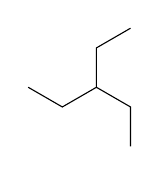
\begin{tikzpicture}
  \begin{scope}[scale=0.5]\draw
  (0,0)--++(0,1) --++({-cos(90+120)},{-sin(90+120)})
  (0,0)--++({cos(90+120)},{sin(90+120)})--++({-cos(90+240)},{-sin(90+240)})
  (0,0)--++({cos(90+240)},{sin(90+240)})--++(0,-1)
  ;\end{scope}
\end{tikzpicture} -- зигзаг, результирующий будет сдвинут по фазе относительно
фазы A. На рисунке равноплечный зигзаг, бывает неравноплечный зигзаг. Зигзаги
бывают также обратными

\begin{tikzpicture}
  \begin{scope}[scale=0.5]\draw
    (0,0)--++(0,1) --++({-cos(90+240)},{-sin(90+240)})
    (0,0)--++({cos(90+120)},{sin(90+120)})--++(0,-1)
    (0,0)--++({cos(90+240)},{sin(90+240)})--++({-cos(90+120)},{-sin(90+120)})
    ;\end{scope}
\end{tikzpicture}
Сдвиг фазы 30\% -- равноплечный зигзаг, если зигзаг неравноплечный, то сдвиг
фаз может быть от $0^\circ$ до $60^\circ$

Треугольники бывают правые и левые.
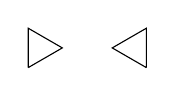
\begin{tikzpicture}\begin{scope}[scale=0.5]\draw
  (0,0)--++(0,1)--++({cos(-30)},{sin(-30)})--++({cos(210)},{sin(210)})
  (3,0)--++(0,1)--++({cos(210)},{sin(210)})--++({cos(-30)},{sin(-30)})
  ;\end{scope}
\end{tikzpicture}


Существует соединение обмоток по схеме шестиугольника
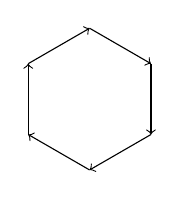
\begin{tikzpicture}\begin{scope}[scale=0.9]
%    \path (0,0) node (a0){} --++(0,1)node(a1){};
    \draw[->] (0,0)--++(0,1) coordinate (a1);
    \draw[->] (a1)--++({cos(30)},{sin(30)}) coordinate (a2);
    \draw[->] (a2)--++({cos(-30)},{sin(-30)}) coordinate (a3);
    \draw[->] (a3)--++(0,-1) coordinate (a4);
    \draw[->] (a4)--++({-cos(30)},{-sin(30)}) coordinate (a5);
    \draw[->] (a5)--++({-cos(-30)},{-sin(-30)})
    ;\end{scope}
\end{tikzpicture}

Звезда и треугольник энергетически эквивалентны друг другу. Никакими
силами не определить разницу между
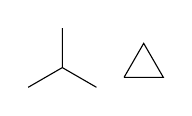
\begin{tikzpicture}
  \begin{scope}[scale=0.5]
    \coordinate (o) (0,0);
    \coordinate (o1) ({2+1/2*cos(90+120)},{1/2*sin(90+120)});
    \draw (o)--++(0,1)
          (o)--++({cos(90+120)},{sin(90+120)})
    (o)--++({cos(90+240)},{sin(90+240)})
    ({2+1/2*cos(90+120)},{1/2*sin(90+120)})
    --++({cos(60)},{sin(60)})--++({cos(-60)},{sin(-60)})--++(-1,0)
    ;      
    \end{scope}
  \end{tikzpicture}

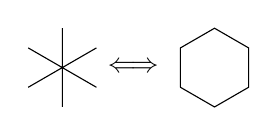
\begin{tikzpicture}
  \begin{scope}[scale=0.5]
    \coordinate (o) (0,0);
    \draw (o)--++(0,1)
    (o)--++({cos(30)},{sin(30)})
    (o)--++({cos(150)},{sin(150)})
    (o)--++({cos(210)},{sin(210)})
    (o)--++(0,-1)
    (o)--++({cos(330)},{sin(330)})
    
    (3,-0.5)--++(0,1)--++({cos(30)},{sin(30)})--++({cos(-30)},{sin(-30)})--++
    (0,-1)--++({-cos(30)},{-sin(30)})--++({-cos(-30)},{-sin(-30)})

    (1.8,0) node {$\Longleftrightarrow$};
     
  \end{scope}
  \end{tikzpicture} -- также никакими силами не определить разницу

\begin{tikzpicture}\begin{scope}[scale=0.5]\draw
    (0,2)--++(0,1)
    (0,2)--++({cos(120+90)},{sin(120+90)})
    (0,2)--++({cos(240+90)},{sin(240+90)})

    (-1,0)--++(0,1)
    (-1,0)--++({cos(120+90)},{sin(120+90)})
    (-1,0)--++({cos(240+90)},{sin(240+90)})

    (1.2,0)--++(0,-1)
    (1.2,0)--++({-cos(120+90)},{-sin(120+90)})
    (1.2,0)--++({cos(-240+90)},{-sin(240+90)})
    % core
    (-1.5,1.2) rectangle (1.8,1.22)
    %
    (-1,0)--(1.2,0);
    \draw[thin,<-] (2,0)--(3.5,0) node[right]{6-фазная звезда}
    ;\end{scope}\end{tikzpicture}

Был 4-й провод ``нулевой'', но оборвался. Если на трансформаторе написано
6кВт это фазное или линейное напряжение. 380В напряжение меряют по междуфазному.
Терминология -- трансформаторы называют по большему напряжению. ``0''
может быть физический, а может быть искусственно созданный.

\begin{circuitikz}\draw
  (0,2.5)--(5,2.5)
  (0,2)--(5,2)
  (0,1.5)--(5,1.5)
  (1,0)to[european resistor](1,1)to[short,-*](1,1.5)
  (2,0)to[european resistor](2,1)to[short,-*](2,2)
  (3,0)to[european resistor](3,1)to[short,-*](3,2.5)
  (1,0)--(4,0)to[lamp](4,1)to[short,-*](4,1.5);
  \draw[thin,<-] (2,-0.1)--(2,-0.6) node[below]
       {это искусственно созданный ``0''}
       ;\end{circuitikz}

Так же искусственный ноль можно сделать в 6-ти фазной сети, подключив 6 чайников,
чего хотите.
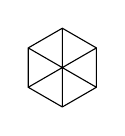
\begin{tikzpicture}
  \begin{scope}[scale=0.5]\draw
    (0,0)--++(0,1)
    (0,0)--++({cos(30)},{sin(30)})
    (0,0)--++({cos(-30)},{sin(-30)})
    (0,0)--++(0,-1)
    (0,0)--++({cos(150)},{sin(150)})
    (0,0)--++({cos(210)},{sin(210)})
    %
    (0,-1)--++({cos(30)},{sin(30)})--++(0,1)--++({cos(150)},{sin(150)})--++
    ({cos(210)},{sin(210)})--++(0,-1)--++({cos(-30)},{sin(-30)})
    ;\end{scope}
\end{tikzpicture}

Как получить 9 фаз?

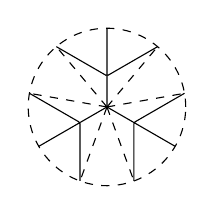
\begin{tikzpicture}\draw
  (0,0)--++(0,1)
  (0,0)--++({cos(90+120)},{sin(90+120)})
  (0,0)--++({cos(90+240)},{sin(90+240)})
  ({cos(50)},{sin(50)})--++({0.73*cos(90+120)},{0.73*sin(90+120)})
  ({cos(130)},{sin(130)})--++({0.73*cos(90+240)},{0.73*sin(90+240)})
  ({cos(170)},{sin(170)})--++({0.73*cos(90+240)},{0.73*sin(90+240)})
  ({cos(250)},{sin(250)})--++(0,0.73)
  ({cos(290)},{sin(290)})--++(0,0.73)
  ({cos(10)},{sin(10)})--++({0.73*cos(90+120)},{0.73*sin(90+120)});
  \draw[dashed]
  (0,0)--({cos(50)},{sin(50)})
  (0,0)--({cos(130)},{sin(130)})
  (0,0)--({cos(170)},{sin(170)})
  (0,0)--({cos(250)},{sin(250)})
  (0,0)--({cos(290)},{sin(290)})
  (0,0)--({cos(10)},{sin(10)})
  (0,0)circle(1cm)
  ;\end{tikzpicture}

это и есть эквивалентная ЭДС. Здесь картина симметричная. Если делать 4 фазы,
получится несимметричная ЭДС.

$r_\phi$ -- эквивалентное фазное -- это сопротивление К.З., учитывающее
индуктивность рассеяния первичной и вторичной обмоток трансформатора.
\begin{tikzpicture}
  \draw[thin,->] (0,0)--(3.2,0) node[right] {$U$};
  \draw[thin,->] (0,0)--(0,2.1) node[left] {$I$};
  \draw (1,0)--(1,2)
  (1,0)--({1+2*cos(60)},{2*sin(60)})
  ({1+1.5*cos(60)},{1.5*sin(60)}) arc(60:90:1.5)
  ;\end{tikzpicture}

\begin{circuitikz}\draw
  (0,3.83)--(0,4)--(7,4)--(7,3.5)
  (0,3.5) circle(0.33)
  (0,3.5) node {$e_1$}
  (0,3.17)--(0,3)to[european resistor,l={$r_\phi$}](0,2)to[L,l={$L_\phi$}](0,1)to[Ty,mirror](0,0)
  (0,0)--(0,-0.33)--(0.3,-0.33)
  (1.8,-0.33)--(3.2,-0.33)
  (4.6,-0.33)--(5,-0.33)
  (2,3.83)--(2,4)
  (2,3.5) circle(0.33)
  (2,3.5) node {$e_k$}
  (2,3.17)--(2,3)to[european resistor,l={$r_\phi$}](2,2)to[L,l={$L_\phi$}](2,1)to[Ty,mirror](2,0)
  (2,0)--(2,-0.33)
  (3,3.83)--(3,4)
  (3,3.5) circle(0.33)
  (3,3.5) node {$e_{k\!+\!1}$}
  (3,3.17)--(3,3)to[european resistor,l={$r_\phi$}](3,2)to[L,l={$L_\phi$}]
  (3,1)to[Ty,mirror](3,0)
  (3,0)--(3,-0.33)
  (5,3.83)--(5,4)
  (5,3.5) circle(0.33)
  (5,3.5) node {$e_m$}
  (5,3.17)--(5,3)to[european resistor,l={$r_\phi$}](5,2)to[L,l={$L_\phi$}]
  (5,1)to[Ty,mirror](5,0)
  (5,0)--(5,-0.33)
  %
  (7,1.5)to[L](7,0.5)
  (7,1.5)to[american current source,l_={$E_\textcyrillic{н}$}](7,2.5)
  to[european resistor,l_=r](7,3.5)
  (7,0.5)--(7,-0.66)--(2.5,-0.66)--(2.5,-0.33)
  ;
  \draw[thin,<-] (7.6,1.8)--(8.5,0.5) node[right]
       {$\begin{array}{c}\textcyrillic{может быть}\\
           \textcyrillic{встречно}\\
           \textcyrillic{или согласно}\\
         \textcyrillic{с напряжением}\end{array}$};
  \draw[thin,<->](8,-0.66)--(8,4) node[midway,right] {$u_d,$ $U_d$};
  \draw[loosely dashed] (0.5,-0.33)--(1.6,-0.33)
  (3.4,-0.33)--(4.4,-0.33);
\end{circuitikz}

Какая полярность нагрузки считается положительной?

\begin{circuitikz}\draw
  (0,0)circle(0.33)
  (0,0)node{e}
  (-0.33,-0.33)node{+}
  (-0.33,0.33)node{-};
  \draw[thin,<-] (0.5,0)--(1.5,0) node[right]{положительная}
  ;\end{circuitikz}
положительная,согласная с током на нагрузке. И называют её противоЭДС

\begin{circuitikz}[]
  \draw
  
  (0,0)to[american current source,v^=$ $](0,1)
  (0.5,0.2)to[short,i_=i](0.5,0.8)
  ;\end{circuitikz}

Если среднее, то $U_d$, если на осциллографе, то $u_d$.

\begin{circuitikz}
  \draw
  (1,3) --(2,3) node[right] {-}
  (1,0.5)--(2,0.5) node[right]{+};
  \draw (1.5,0.5)--(1.5,3) node[midway,left] {$L_\textcyrillic{н}$};
  \draw[->](0.3,0)--(1,0) node[right] {$I_d$ $i_d$};
  \draw (2.5,1.75)circle(0.33);
  \draw (2.85,2.08) node[right] {-};
  \draw (2.83,1.42) node[right] {+};
  \draw[<-] (3,1.75)--(3.8,1.75) node[right] {противоЭДС};
\end{circuitikz}  

Пульсирующий постоянный ток -- это плохой ток. Чтобы уменьшать пульсации
в основном применяют индуктивные фильтры. Обычно индуктивности в обмотке
мотора может быть достаточно. Переменная составляющая может быть мала.

\begin{circuitikz}\draw
  (0,0)to[L,l_={$\chi$}](2,0)
  (0.5,0.25)rectangle(1.5,0.27)
  (1,0.5) node[right]{$L_\Phi$}
  ;\end{circuitikz}
  
Индуктивность может насыщаться, со стальным сердечником можно 
$\displaystyle \frac{\Psi}{I}$, а большой поток, когда есть $L$ фильтра.

$$
\begin{array}{c}
R_d = (R_\textcyrillic{н}+R_\Phi)\\
L_d = (L_\textcyrillic{н}+L_\Phi)
\end{array}
$$

Допущения: В самой сети фазы одинаковы, симметричныю
% http://tex.stackexchange.com/questions/209942/curved-arrows-in-tikz
% http://www.texample.net/tikz/examples/borrowers-and-lenders/
Доказываем:

\begin{circuitikz}
\draw[domain=-0.5:0.5,samples=100]
plot (\x, {1.3+0.5*cos((\x*(pi/6)/0.5)*180)});
\draw[domain=0.5:1.5,samples=100]
plot (\x, {1.3+0.5*cos(((\x+1)*(pi/6)/0.5)*180)});
;
\draw
(0,1)to[Do,v^>={$ $}](0,0) node[below] (n0) {}
(1,1)to[Do,v^<={$ $}](1,0)
;
\draw[thin,<-] (1.4,0.8)--(2,1)node[right] (n1) {предполагаем}
edge[bend left=45,->] node[midway,below right]{значит} (n0.south);
\end{circuitikz}

Если пренебречь сопротивлениями $L_\phi$ и $r\phi$ то должен закрыться 
вентиль.

\subsection{нулевая однофозная однополупериодная схема}

Сеть пришла с $m$ проводами. 
\begin{circuitikz}\draw
(0,0) node[anchor=east]{} to[short,o-](3,0)
to[european resistor,l_=$Z_\textcyrillic{н}$](3,2)
(1,2) to[short,-o](0,2) node[anchor=east]{}
(1,2)to[Do](2,2)to[short](3,2)
(0,1)node{$\sim$}
;\end{circuitikz}

Как считать $\chi$ пока не говорим. В нашем случае $m=1$.
У неё неи ни предыдущей ни последующей фазы. Фильтрация здесь невозможна
потому что нет постоянной ЭДС, нет постоянного тока. Обязательно будет
\underline{перерыв} в токе. <положительная больше отрицательного> 

%http://tex.stackexchange.com/questions/207770/transformers-in-circuitikz
\begin{circuitikz}[american]\draw
(0,0) node[transformer core](T){}
(T.B1)to[D](2.5,0)
(T.B2)to[D](2.5,-2.1)to[short,-*](2.5,0)
(T.B1)to[short](2.5,0) % вентили всегда прочерктваются по ГОСТу
(T.B2)to[D](2.5,-2.1)
($(T.B1)!0.508!(T.B2)-(0.7,0)$) --++(4,0)
to[european resistor,l_=$Z_\textcyrillic{н}$]($(T.B1)+(3.3,0)$)--++(-2,0)
;
\draw[thin,<-] (2,0.2)--(2.5,0.5) 
node[right]{вентили всегда прочерктваются по ГОСТу};
\end{circuitikz}

Схема, вообще говоря, двухфазная. 
Называется однофазная двухполупериодная.
$m=2$! -- эквивалентное число фаз равно двум.

Несимметричная двухфазная система 
\begin{tikzpicture}
\draw[->] (0,0)--(0,1.5);
\draw[->] (0,0)--(1,0);
\end{tikzpicture}

Симметричная, когда модули одинаковые. В трехфазной системе симметричных
не одна , а три ``нулевая'', ``прямая'' и ``обратная''. У 5-фазных
5 штук симметрий.

Симметричная фазная система это такая, модули составляющих одинаковые
и углы между составляющими одинаковы.

$\displaystyle \frac{2\pi}{m}$ -- ``прямая'' симметрия.

$\displaystyle -\frac{2\pi}{m}$ -- ``обратная'' симметрия.

$0$ - нулевая.

\begin{circuitikz}[american]\draw
(0,0) node[transformer core](T){}
(T.B1)to[D](3,0)
(T.B2)to[D](3,-2.1)to[short,-*](3,0)
(T.B1)to[short](3,0) % вентили всегда прочерктваются по ГОСТу
(T.B2)to[D](3,-2.1)
($(T.B1)!0.508!(T.B2)-(0.7,0)$) --++(4.5,0)
to[european resistor,l_=$Z_\textcyrillic{н}$]($(T.B1)+(3.8,0)$)--++(-2,0)
(0, 0.5) node[right]{2 вектора, угол между ними $180^\circ$};
\draw[->](0.6,-0.65)arc(180:90:0.4)--(1.3,-0.25) node[right]
{$\frac{1}{2}$};
\draw[->](0.6,-1.45)arc(180:270:0.4)--(1.3,-1.85) node[right]
{$\frac{1}{2}$};
\draw[thin,<-](2,-1.5)--(3.5,-2.8)node[right]{плохое использование мощности
трансформатора};
\end{circuitikz}

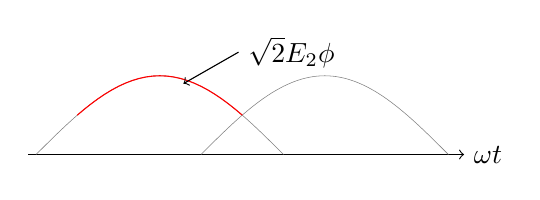
\begin{tikzpicture}\begin{scope}
\draw[thin,->] (-pi/2-0.1,0)--(pi/6+pi+0.2,0) node[right]{$\omega t$};
\draw[domain=-pi/2:pi/2,help lines,smooth]
plot(\x, {cos(\x r)});
\draw[domain=pi/6:pi/6+pi,help lines,smooth]
plot(\x, {cos((\x-2/3*pi) r)});
\draw[domain=-pi/3:pi/3,red]
plot(\x, {cos(\x r)});
\draw[<-](0.3,0.9)--(1,1.3) node[right] {$\sqrt{2}E_2\phi$};
\end{scope}
;\end{tikzpicture}

